
\chapter{Testy jakościowe i wydajnościowe}

W bibliotekach wykorzystywanych przez programistów równie ważna jak
bogata funkcjonalność czy łatwość użycia jest stabilność działania
i pewność, że błąd w~wykonaniu aplikacji nie leży po stronie biblioteki.
W związku z tym istotne jest pokrycie kodu biblioteki zestawem testów
zarówno jednostkowych jak i akceptacyjnych, które zostały opisane
w niniejszym rozdziale.

Oprócz testów jakościowych przeprowadzone zostały testy wydajnościowe,
które pozwoliły określić wydajność biblioteki w obecnym stanie implementacyjnym
oraz określić wpływ rodzaju przetwarzania na zasadność prowadzenia
przetwarzania rozproszonego.


\section{Testy jakościowe}

\label{sec:Testy-jako=00015Bciowe}Testy jakościowe pozwalają na sprawdzenie
konkretnych funkcji biblioteki w spreparowanym środowisku testowym.
Testy jednostkowe i integracyjne, działają w środowisku Microsoft
Unit Test Framework \cite{Microsoft-Unit-Test-Framework-for-Managed-Code}
zintegrowanym ze środowiskiem Visual Studio. Dodatkowo wykorzystana
została biblioteka Shoudly \cite{Shouldly} do zapisu asercji oraz
Moq \cite{Moq} do tworzenia atrap obiektów.


\subsection{Testy jednostkowe}

Testując niektóre funkcje biblioteki wskazane było sprawdzenie ich
zachowania abstrahując od ich zależności. W tym celu równolegle z
tworzonym kodem powstawały testy jednostkowe. Należy również zwrócić
uwagę, że testy jednostkowe wykonują się znacznie szybciej od testów
integracyjnych, co pozwala znacząco skrócić czas wykrycia oraz poprawy
ewentualnych błędów. Poniżej przedstawiono przykładowe przypadki testowe:
\begin{itemize}
\item \dcsname{lokalny wykonawca} -- operacja \dcscode{Join} z określonym
limitem czasu oczekiwania na jej zakończenie,
\item \dcsname{zdalny wykonawca} -- testy operacji \dcscode{Pulse} z użyciem
atrapy obiektu (ang.~\dcsemph{mock object}),
\item usługa \dcsname{zdalnego wykonawcy} -- wykonanie metody z użyciem
zserializowanego uchwytu, przechwytywanie wyjątków w kodzie użytkownika,
zwracanie statystyk obciążenia węzła oraz testy z użyciem zmienionej
implementacji interfejsu (ang.~\dcsemph{fake object}) -- operacji
\dcscode{Join} (synchronicznej i asynchronicznej), rzucenia przechwyconego
w kodzie użytkownika wyjątku w momencie wykonywania operacji \dcscode{Join},
wstrzykiwania zależności \dcscode{IBluepathCommunicationFramework}
(przez podmianę oraz przez dodanie brakującego parametru),
\item \dcsname{wątek rozproszony} -- wykonanie z użyciem \dcsname{lokalnego wykonawcy},
\dcsname{zdalnego wykonawcy} (potrzebne usługi, tj. \dcscode{IRemoteExecutorService}
i \dcscode{IScheduler} zostały zasymulowane za pomocą atrap obiektów,
użyto też \dcsname{zarządcy połączeń} w trybie bez wywołań zwrotnych),
głębokie kopiowanie parametrów wywołania,
\item planista \dcscode{ThreadNumberScheduler} -- test sprawdza, czy następuje
wybór najmniej obciążonego węzła spośród zasymulowanych,
\item z uwagi na użycie własnej klasy \dcscode{ServiceUri} jako klucza
w słowniku, testowano też taki scenariusz.
\end{itemize}

\subsection{Testy integracyjne}

W celu przetestowania działania funkcji takich jak przesyłanie klas
jako parametrów wskazane jest stworzenie testów integracyjnych. Ich
zadaniem jest przetestowanie nie tylko logiki wykonywanego kodu, ale
również wykrycie problemów jakie mogą się pojawić w związku z działaniem
w środowisku sieciowym (np. wymagane uprawnienia do utworzenia usługi
nasłuchującej, serializacja obiektów).

Jednym z problemów związanych z testami integracyjnymi jest potrzeba
stworzenia środowiska testowego. W momencie gdy zachodzi potrzeba
uruchomienia zewnętrznego programu (np. Redisa) system operacyjny
nie dostarcza narzędzi, które pozwoliłyby określić nie tylko czy dany
proces jest już uruchomiony, ale również czy skończył on proces inicjalizacji.
Należy również zwrócić uwagę, że testy nie powinny być od siebie zależne
-- a więc efekt wykonania jednego testu nie powinien mieć wpływu na
inne testy. Aby tego uniknąć, każdy test został wyposażony w taki
zestaw parametrów, który pozwoli mu się wykonać niezależnie od innych
(np. port na którym ma nasłuchiwać usługa \dcsname{Bluepath}).

W ramach testów integracyjnych przetestowane zostały następujące aspekty:
\begin{itemize}
\item \dcsname{wątki rozproszone} -- zachowanie systemu w wyniku próby
wykonania metod akceptujących różne typy parametrów i zwracające wyniki
różnego typu -- tablice, klasy (także generyczne), delegaty, a także
obsługa wyjątków w kodzie użytkownika oraz w przypadku nieprawidłowego
wywołania; test obejmował także wykonanie metody z biblioteki napisanej
w języku F\#,
\item \dcsname{zarządca połączeń} -- pobieranie listy dostępnych węzłów
z \dcsname{usługi odnajdywania węzłów} i aktualizowanie swojej
lokalnej kopii listy (dodawanie nowych węzłów i usuwanie wyrejestrowanych),
pobieranie informacji o obciążeniu węzłów zarejestrowanych w klastrze,
\item \dcsname{pamięć rozproszona} -- testy zapisu i odczytu obiektów
(także jako operacji zbiorczych),
\item \dcsname{zamki rozproszone} -- pobieranie i zwalnianie zamków (także
z limitem czasu), budzenie wątków czekających na zamkach,
\item a także testy struktur danych i obiektów zbudowanych na bazie \dcsname{pamięci rozproszonej}
-- lista, słownik, licznik.
\end{itemize}

\section{Testy wydajnościowe}

Ważną częścią tworzenia biblioteki programistycznej jest zweryfikowanie
jej zachowania w przykładowych zastosowaniach. Pozwala to zweryfikować
słuszność przyjętych założeń i rozwiązań. 

Przy okazji weryfikacji działania biblioteki \dcsname{Bluepath} przeprowadzone
zostały testy wydajnościowe, zestawiające efekt wykonania przetwarzania
w klastrze w stosunku do przetwarzania na pojedynczym procesorze oraz
porównanie dostarczonych przykładowych algorytmów szeregowania zadań.


\subsection{Środowisko }

Środowisko do przeprowadzenia testów wydajnościowych zostało przygotowane
w~oparciu o platformę Microsoft Azure \cite{Microsoft-Azure}. Klaster
składał się z 7 maszyn wirtualnych -- na sześciu z nich działały usługi
systemu Bluepath pod kontrolą systemu operacyjnego Windows Server
2012 R2 Datacenter (wydanego 17 czerwca 2014 r.), a na jednej maszynie
uruchomiony został host \dcsname{pamięci rozproszonej} Redis pod
kontrolą systemu operacyjnego Ubuntu Server 14.04 LTS (wydanego 20
czerwca 2014 r.). Maszyny różniły się konfiguracją sprzętową w zależności
od przeznaczenia:
\begin{itemize}
\item węzeł inicjujący przetwarzanie był typu \dcsname{Medium VM (Basic A2)}
i posiadał 2~wirtualne rdzenie AMD Operton 1,6 GHz i 3,5 GB pamięci
operacyjnej, 
\item węzły obliczeniowe były typu \dcsname{Small VM (Basic A1)} dysponowały
po 1 wirtualnym rdzeniu AMD Opteron 1,6 GHz i 1,75 GB pamięci operacyjnej, 
\item węzeł hostujący usługę Redis była to instancja typu \dcsname{Large VM (Basic A3)}
posiadająca cztery rdzenie AMD Opteron 1,6 GHZ i 7 GB pamięci operacyjnej. 
\end{itemize}
Szczegóły konfiguracji zestawiono w tabeli \ref{tab:performance-Konfiguracja-testowego-klastra}.
Maszyny wirtualne wchodzące w~skład klastra połączone zostały w wirtualną
sieć, w której wyłączone były zapory sieciowe, a komunikacja odbywała
się z użyciem prywatnych wewnętrznych adresów IP (tzw. \dcsname{DIP},
przydzielony automatycznie przez Windows Azure z użyciem DHCP). 

\begin{table}
\centering{}\protect\caption{\label{tab:performance-Konfiguracja-testowego-klastra}Konfiguracja
testowego klastra}
\begin{tabular}{|c|c|c|c|c|}
\hline 
Nazwa maszyny & Typ instancji & Liczba rdzeni & Pamięć RAM & System operacyjny\tabularnewline
\hline 
\hline 
Master & A2 & 2 & 3,5 GB & Windows Server\tabularnewline
\hline 
Slave1 & A1 & 1 & 1,75 GB & Windows Server\tabularnewline
\hline 
Slave2 & A1 & 1 & 1,75 GB & Windows Server\tabularnewline
\hline 
Slave3 & A1 & 1 & 1,75 GB & Windows Server\tabularnewline
\hline 
Slave4 & A1 & 1 & 1,75 GB & Windows Server\tabularnewline
\hline 
Slave5 & A1 & 1 & 1,75 GB & Windows Server\tabularnewline
\hline 
Redis & A3 & 4 & 7 GB & Ubuntu Server\tabularnewline
\hline 
\end{tabular}
\end{table}


Do dystrybucji nowych wersji bibliotek systemu Bluepath na wszystkie
maszyny w klastrze przygotowany został skrypt PowerShell przedstawiony
na listingu \ref{lis:performance-Skrypt-dystrybuuj=000105cy-biblioteki}.
Wykorzystuje on opisany w punkcie \ref{sec:implementation-Skrypt-Send-Folder}
skrypt \dcspath{Send-Folder}.

\inputencoding{latin2}\begin{lstlisting}[caption={Skrypt
dystrybuuj�cy biblioteki w klastrze},label={lis:performance-Skrypt-dystrybuuj=000105cy-biblioteki},breaklines=true,language=bash,numbers=left]
.\Send-Folder.ps1 -server [adres w�z�a 1] -user [nazwa u�ytkownika] 
  -password [has�o] -source [folder �r�d�owy] -destination [folder docelowy]
...
.\Send-Folder.ps1 -server [adres w�z�a n] -user [nazwa u�ytkownika] 
  -password [has�o] -source [folder �r�d�owy] -destination [folder docelowy]
\end{lstlisting}
\inputencoding{utf8}


\subsection{Generowanie słownika prefiksów}

Jednym z algorytmów wykorzystanych do pomiaru wydajności był algorytm
tworzący prefiksy na potrzeby przeprowadzenia operacji uzupełniania
tekstu opisany w~punkcie \ref{sub:zastosowania-autocomplete-Wczytywanie-danych}.
Dla określonej liczby dokumentów znajdujących się w \dcsname{pamięci rozproszonej}
pomiar czasu przetwarzania był powtarzany dziesięć razy. Wykres \ref{fig:performance-Generowanie-prefixow}
przedstawia porównanie uśrednionych czasów generowania słownika prefiksów
na pojedynczym węźle oraz w klastrze. Dla zbioru 10000 dokumentów
udało się uzyskać prawie dwukrotne przyspieszenie w stosunku do przetwarzania
na pojedynczej maszynie. Warto również nadmienić, że w algorytmie
testującym wprowadzono mechanizm okresowo czyszczący lokalną pamięć
prefiksów ze względu na wyczerpywanie się pamięci w przypadku przetwarzania
na pojedynczym węźle.

\begin{figure}
\centering{}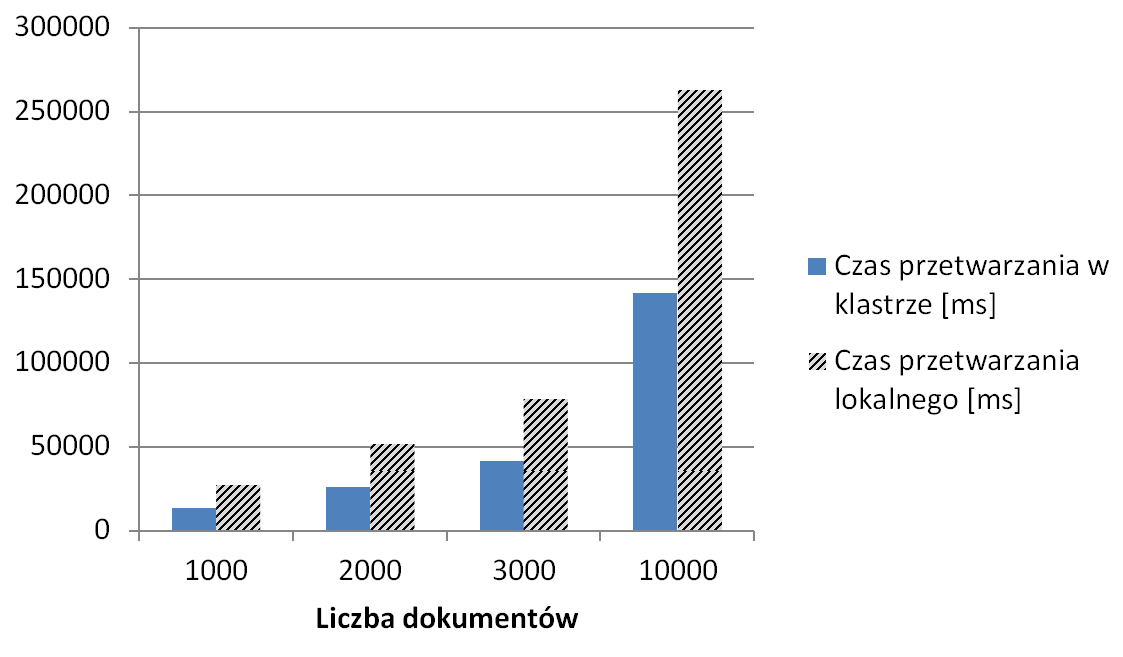
\includegraphics[scale=0.5]{images/prefixy-6}\protect\caption{\label{fig:performance-Generowanie-prefixow}Porównanie czasu generowania
słownika prefiksów }
\end{figure}



\subsection{Obliczanie przybliżenia liczby $\pi$}

\label{sub:performance-Obliczanie-przyblizenia-Pi}Kolejnym algorytmem,
przy pomocy którego zmierzono zysk związany z zastosowaniem biblioteki
Bluepath było obliczanie przybliżenia liczby $\pi$ metodą przedstawioną
w punkcie \ref{sec:Przykladowe-zastosowania-liczba-pi}. Wykres \ref{fig:performace-Por=0000F3wnanie-czasu-obliczania-pi}
przedstawia porównanie uśrednionych czasów przetwarzania na pojedynczym
węźle oraz w klastrze w zależności od rozmiaru instancji. Czas został
przedstawiony w skali logarytmicznej. 

\begin{figure}
\centering{}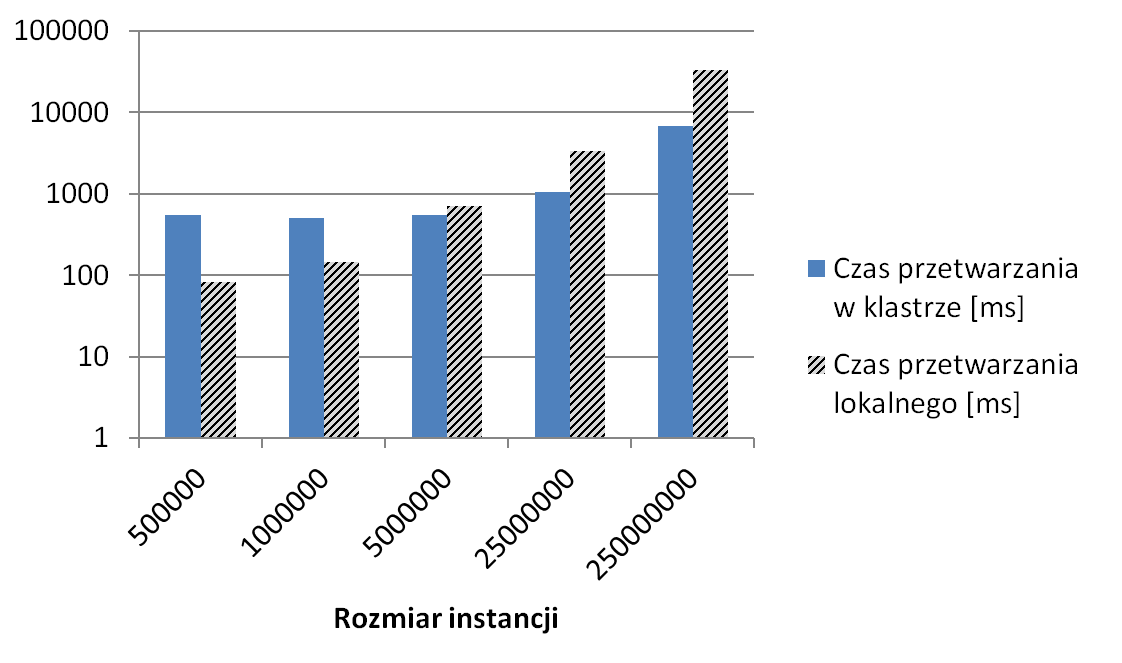
\includegraphics[scale=0.5]{images/pi-5-machines}\protect\caption{\label{fig:performace-Por=0000F3wnanie-czasu-obliczania-pi}Porównanie
czasu obliczania przybliżenia liczby $\pi$}
\end{figure}


Dla dużych instancji przetwarzanie przy pomocy biblioteki Bluepath
jest dużo szybsze niż przetwarzanie na pojedynczym węźle. Jednak dla
małych instancji narzut generowany przez bibliotekę sprawia, że przetwarzanie
w klastrze staje się mniej efektywne niż przetwarzanie lokalne. Można
to również zauważyć na wykresie \ref{fig:performace-Przyspieszenie-pi}.
Przedstawia on przyspieszenie uzyskane w związku z zastosowaniem biblioteki
Bluepath do przetwarzania w klastrze w stosunku do przetwarzania na
pojedynczym węźle. 

\begin{figure}
\centering{}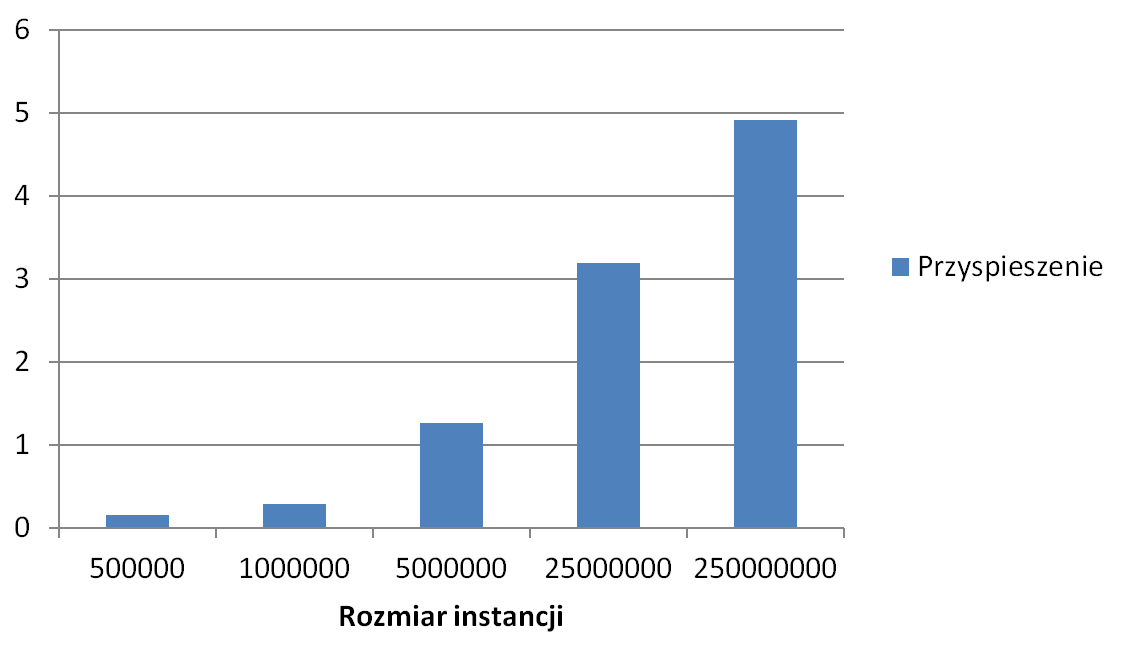
\includegraphics[scale=0.5]{images/pi-5-speedup}\protect\caption{\label{fig:performace-Przyspieszenie-pi}Przyspieszenie w stosunku
do przetwarzania lokalnego}
\end{figure}


Narzut widoczny na obu wykresach jest częstym zjawiskiem w systemach
rozproszonych i wynika z konieczności przeprowadzenia komunikacji
sieciowej.
